\section{Methodology}

We explain the multi-agent environment for this study, our proposed detection and mitigation methods for problem drift, and the datasets and metrics.

\begin{figure*}[ht]
    \centering
    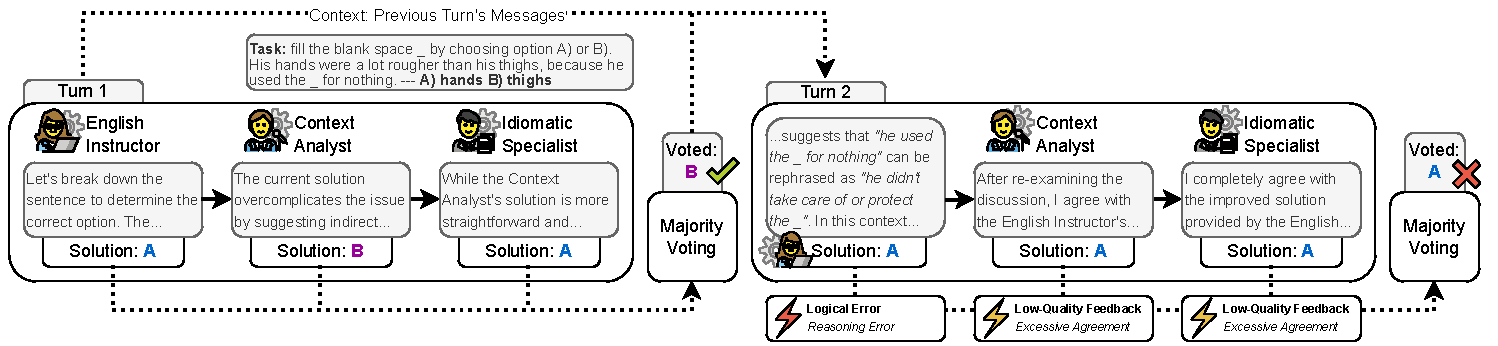
\includegraphics[width=0.99\linewidth]{figures/other_charts/discussion_large.drawio.pdf}
    \caption{Example of problem drift in MAD. The \textit{English instructor} induces a logical error in the discussion. The other agents agree without skepticism, leading to the wrong solution and problem drift.}
    \label{fig:discussion_turn}
\end{figure*}

\subsection{Debate Setup} \label{sec:setup}
We define three components for running MAD: an interface for agents, discussion paradigms, and the decision-making protocol.
For each task, we create three agents with distinct \textbf{expert personas} \citep{XuYLW23a, ShiZWW23a}. 
We choose three agents as a hyperparameter following previous works \citep{ChenSB24a, YinSCG23a}.
These personas are automatically generated by \href{https://huggingface.co/meta-llama/Llama-3.1-70B-Instruct}{\textit{Meta-llama/Meta-Llama-3.1-70B-Instruct}} \citep{GrattafioriDJP24a} and induce a set of preferences (e.g., law attorney), which varies according to the task and sample (examples and details are in \Cref{app:examples}).
Second, we run a total of \textbf{seven turns} of conversation between the agents.
We find that in 99\% of cases, agents reach a first agreement within the first two turns.
Thus, we choose seven turns to capture the effects of prolonged agent interaction sufficiently.
This aligns with other setups for MAD \citep{YinSCG23a} and enables our analysis of recovery following problem drift.
Each agent can generate one new message at each turn and indicate their agreement with the current solution.
All agents see the messages of one another.
If an agent disagrees, it proposes a new solution concomitantly.
Finally, we employ two decision-making protocols that other researchers regularly use to ensure that our findings generalize across conversational setups \citep{YinSCG23a, kaesberg2025, YangDKH24}.
\textbf{Voting} is conducted between possible discussed solutions to reach a final solution for that turn \citep{YangDKH24}.
Following prior work, agents have access to one previous turn and the previously voted solution \citep{PagnoniBT21a, ZhangZ20b}.
A visual overview of the process is presented in \Cref{fig:discussion_turn}.
\textbf{Consensus} involves each agent directly modifying the current draft at their turn \citep{YinSCG23a}.
A visual overview of the process can be found in \Cref{fig:discussion_turn_consensus} of \Cref{app:overview_of_consensus}.

% We choose voting \citep{YangDKH24} over consensus \citep{ChenSB24a} for decision-making because we require a definitive solution at the end of each turn that is not biased towards the order of agent contributions.
% Voting allows for a direct performance measurement after each turn.
%To test whether our findings and mitigation methods generalize to other setups, we perform an additional experiment using consensus-based decision-making by the end of this study.
% \begin{figure}[t]
%     \centering
%     \includegraphics[width=0.99\linewidth]{figures/other_charts/discussion.drawio.pdf}
%     \caption{Relevant context for the generation of the agent message E (green). Dashed lines indicate the components that are the relevant context.}
%     \label{fig:discussion_turn}
% \end{figure}

We conduct our experiments using \href{https://huggingface.co/meta-llama/Llama-3.1-70B-Instruct}{\textit{Meta-llama/Meta-Llama-3.1-70B-Instruct}} on eight NVIDIA A100 GPUs, and \href{https://huggingface.co/Qwen/Qwen2-7B-Instruct}{\textit{Qwen/Qwen2-7B-Instruct}} on two NVIDIA A100 GPUs with 40 GB each.
Detailed information about the framework \citep{becker2025mallmmultiagentlargelanguage}, parameters, and prompts is available in \Cref{app:framework,app:parameters,app:prompts}.
We report our main results using \textit{Llama-3.1} and \textit{Voting} but also include results for \textit{Qwen2} and \textit{Consensus} to ensure the generalizability of our findings.
Our goal is to show that problem drift and \metric\ are not exclusive to the specific design of a multi-agent system and apply to any MAD with intermediate solutions.
As the framework\footnote{\url{https://github.com/Multi-Agent-LLMs/mallm}} and the code\footnote{\url{https://github.com/jonas-becker/problem-drift}} are open source, the exact settings can be investigated, and all experiments can be reproduced.


% \subsection{Reason Identification} \label{sec:dataset}
% We follow a two-step approach to identify the reasons for problem drift.
% Multi-agent conversations can grow large and require a complex understanding of discourse relations.
% Thus, we first create a set of error types by automatically generating them from a large set of drifting conversations using \textit{meta-llama/Meta-Llama-3.1-70B-Instruct} and summarizing with ChatGPT-4o\footnote{Version: 3rd of December 2025}.
% Second, we ask eight human experts to annotate and explain a total of 170 drifting samples to identify the relevance of each error type as well as additional reasons.
% For both steps (systematic and human assessment), we extract the relevant part of the discussion to keep context length manageable, i.e., the three messages of the turn right before the drift and the three messages that cause the problem drift.
% We can do this because, during the discussion, the agent's context memory is also limited to one turn.
% The final list of reasons is provided in \Cref{tab:reasons}.
% A more detailed explanation of the two-step annotation procedure can be read in \Cref{app:dataset_annotation}.
% We publicly release the produced dataset with 170 samples called \textbf{DriftEval} together with the human annotations to our repository.

\subsection{Mitigation Setup}
% After knowing about the existence of problem drift and possible reasons that cause it, the next step is to answer whether and how problem drift can be mitigated.
A natural question from our newly proposed definition of problem drift is whether we can mitigate it even when unsure about its presence (at test-time).
%We detail our detection and mitigation strategy.
%both when the occurrence of problem drift is known (training) and also at test time without gold labels.
%We test two mitigation methods (i.e., \textit{Regenerate}, \policy) and compare the test-time detection of problem drift by an ideal oracle and \judge.

\subsubsection{Detection with \judge}
We aim to identify the occurrence of problem drift at test-time when gold labels are unknown.
%The \textbf{Oracle} setting has precise information about when problem drift occurs because gold labels are known. Thus, we use it to evaluate detection strategies against it.
%Our newly proposed \judge\ detects problems occurring at test-time when gold labels are unknown.
We propose a first baseline to detect problem drift inspired by LLM-as-a-judge \citep{ZhengCSZ23}, which receives a focal turn's and a consecutive turn's solution to assess whether problem drift occurs.
% We provide the immediate previous and current voted solution to the judge rather than the complete conversation as long contexts are computationally prohibitive in our setup \citep{GuJST25}.
To ensure that our results come from architectural changes instead of model capabilities, we refrain from using a powerful fine-tuned model as our judge.
We instead use the same model as for the agents with \judge.
This mitigation concept is independent of our model and could also use lightweight classifiers or models.
%Our goal is for \judge\ to come as close to the Oracle as possible.
%\judge\ detects problem drift at test-time when gold labels are unknown.

\subsubsection{Mitigation Methods}
We propose two mitigation methods to recover debates in the event of drift detection. 
We either \textbf{regenerate} the focal drifting turn or use a \textbf{\policy} agent that provides situational feedback.
%We provide a computational cost analysis for our solution in \Cref{app:compute}.

\paragraph{\textbf{Regenerate.}} We undo the turn suffering from problem drift and regenerate that turn with a non-zero temperature. 
We only regenerate a turn once.

\paragraph{\textbf{\policy.}} We introduce a fourth agent at the end of the drifting turn that provides feedback about how to improve the current conversation and solve the issues leading to problem drift.
%\citet{FuPKL23b} use a policy feedback agent in a game of negotiation, showing that 
\policy\ is inspired by policy feedback agent by \citet{FuPKL23b} and the feedback mechanism used with error types in \citet{kirstein-etal-2025-whats}.
We include the prompt for our feedback generation in \Cref{app:prompts}.


\subsection{Datasets \& Metrics} \label{sec:datasetmetrics}

% Explain which and why we select the datasets specifically
\paragraph{\textbf{Datasets.}} We select ten datasets from four domains: three generative tasks (XSum \citep{NarayanCL18b}, ETPC \citep{KovatchevMS18b}, WMT19 \citep{WikimediaFoundation19}), three reasoning tasks (StrategyQA \citep{GevaKSK21}, WinoGrande \citep{SakaguchiBBC19}, AQUA-RAT \citep{LingYDB17a}), three knowledge tasks (ETHICS \citep{HendrycksBBC23}, MMLU-Pro \citep{WangMZN24}, GPQA \citep{ReinHSP23a}), and one instruction following task (IFEval \citep{ZhouLMB23}).
%The selected tasks vary in complexity (i.e., the required number of reasoning steps) and subjectivity (i.e., characterized by ambiguities or generative problems).
With qualitative assessment, we identify StrategyQA, AQUA-RAT, and MMLU-Pro as \textit{complex} tasks, as they require a higher number of reasoning steps to be solved. 
The generative tasks ETPC, XSum, and WMT19 are characterized by \textit{subjectivity}, due to ambiguities or multiple valid solutions.
As MAD uses large amounts of test-time compute, it has become a common practice to evaluate subsets of datasets to study multi-agent systems \citep{YinSCG23a, ChenSB24a}.
We follow this approach.
Detailed information about the sampling process can be found in \Cref{app:datasets}.
%Previous works conducted multi-agent research on specific applications like story writing \citep{WangMWG23a} or reasoning tasks \citep{YinSCG23a, ChenSB24a}, highlighting where multi-agent systems succeed.
%We differ from these works by selecting a diverse array of tasks to quantify the capabilities of multi-agent LLMs in various scenarios.

\paragraph{\textbf{Metrics.}} We evaluate multiple-choice datasets (i.e., ETHICS, GPQA, MMLU-Pro, StrategyQA, WinoGrande, and Aqua-Rat) by accuracy.
%We provide ROUGE-L \citep{Lin04b} for ETPC and XSum, as well as BLEU \citep{PapineniRWZ02a} for WMT19.
For generative tasks (i.e., ETPC, XSum, and WMT19), we use BERTScore \citep{ZhangKWW19}.
We evaluate IFEval by the ``strict'' accuracy \citep{ZhouLMB23}.

% \paragraph{\textbf{Sampling.}} As MAD uses large amounts of test-time compute, it has become a common practice to evaluate subsets of datasets to study multi-agent systems \citep{YinSCG23a, ChenSB24a}.
% We evaluate samples from each dataset with a 95\% confidence interval and a 5\% margin of error \citep{Cochran53, YinSCG23a, ChenSB24a}.
% Our sample size ranges between 226 to 541 samples per dataset, depending on their size (e.g., 3.1\% of total samples on MMLU-Pro).
% For the small datasets AQUA-RAT and IFEval, we use all available examples.
% To quantify the reliability of the results, we follow \citet{WangPSB24a} and run each experiment three times on randomized subsets and report statistical metrics such as the standard deviation of our results between runs.
% Detailed information about this process can be found in \Cref{app:datasets}.

%\input{tables/good_bad_focus_discussions}

\begin{table*}[t]
\centering
\small
\begin{tabular}{cl|rr|rr|r}
\toprule
& & \multicolumn{1}{c}{\tiny{\# of samples staying at good perf.}} & \multicolumn{1}{c|}{\tiny{\# of samples staying at bad perf.}} & \multicolumn{1}{c}{\tiny{\# of improving samples}} & \multicolumn{1}{c|}{\tiny{\# of worsening samples}} & \multirow{2}{*}{\makecell[r]{\textbf{Total} \\ \textbf{Samples}}} \\
& \textbf{Dataset} & \textbf{$P(\hat{y}^{(r)}, y) > 0.7 \, \forall r$} & \textbf{$P(\hat{y}^{(r)}, y) < 0.7 \, \forall r$} & \textbf{$FOCUS_{1,7}>0$} & \textbf{$FOCUS_{1,7}<0$} & \\
\midrule
\parbox[t]{2mm}{\multirow{3}{*}{\rotatebox[origin=c]{90}{\tiny{Generative}}}} & ETPC & \cellcolor{green!2} 2.0\% \tiny{(22)} & \cellcolor{red!2} 1.9\% \tiny{(21)} & \cellcolor{green!26} 26.5\% \tiny{(287)} & \cellcolor{red!69} 69.5\% \tiny{(753)} & 1.083 \\
& XSum & \cellcolor{green!0} 0.3\% \tiny{(3)} & \cellcolor{red!8} 7.9\% \tiny{(91)} & \cellcolor{green!37} 37.9\% \tiny{(438)} & \cellcolor{red!54} 54.1\% \tiny{(626)} & 1.158 \\
& WMT19 & \cellcolor{green!14} 14.0\% \tiny{(143)} & \cellcolor{red!3} 3.0\% \tiny{(31)} & \cellcolor{green!13} 13.2\% \tiny{(135)} & \cellcolor{red!69} 69.9\% \tiny{(714)} & 1.023 \\
\midrule
\parbox[t]{2mm}{\multirow{3}{*}{\rotatebox[origin=c]{90}{\tiny{Reasoning}}}} & StrategyQA & \cellcolor{green!72} 72.2\% \tiny{(715)} & \cellcolor{red!18} 18.3\% \tiny{(181)} & \cellcolor{green!3} 3.7\% \tiny{(37)} & \cellcolor{red!5} 5.8\% \tiny{(57)} & 990 \\
& WinoGrande & \cellcolor{green!63} 63.4\% \tiny{(561)} & \cellcolor{red!21} 21.3\% \tiny{(188)} & \cellcolor{green!6} 6.8\% \tiny{(60)} & \cellcolor{red!8} 8.6\% \tiny{(76)} & 885 \\
& AQUA-RAT & \cellcolor{green!70} 70.5\% \tiny{(537)} & \cellcolor{red!21} 21.0\% \tiny{(160)} & \cellcolor{green!3} 3.8\% \tiny{(29)} & \cellcolor{red!4} 4.7\% \tiny{(36)} & 762 \\
\midrule
\parbox[t]{2mm}{\multirow{3}{*}{\rotatebox[origin=c]{90}{\tiny{Knowledge}}}} & GPQA & \cellcolor{green!33} 33.2\% \tiny{(225)} & \cellcolor{red!49} 49.9\% \tiny{(338)} & \cellcolor{green!8} 8.1\% \tiny{(55)} & \cellcolor{red!8} 8.7\% \tiny{(59)} & 677 \\
& MMLU-Pro & \cellcolor{green!51} 51.7\% \tiny{(578)} & \cellcolor{red!35} 35.7\% \tiny{(399)} & \cellcolor{green!4} 4.0\% \tiny{(45)} & \cellcolor{red!8} 8.7\% \tiny{(97)} & 1.119 \\
& ETHICS & \cellcolor{green!64} 64.0\% \tiny{(675)} & \cellcolor{red!22} 22.0\% \tiny{(232)} & \cellcolor{green!5} 5.7\% \tiny{(60)} & \cellcolor{red!8} 8.2\% \tiny{(86)} & 1.053 \\
\midrule
\rotatebox[origin=c]{90}{\tiny{IF}} & IFEval & \cellcolor{green!60} 60.4\% \tiny{(898)} & \cellcolor{red!21} 21.7\% \tiny{(323)} & \cellcolor{green!6} 6.1\% \tiny{(90)} & \cellcolor{red!11} 11.8\% \tiny{(175)} & 1.486 \\
\bottomrule
\end{tabular}
\caption{Percentage {\scriptsize (number)} of samples measured across debate rounds $r \in [1,\dots,7]$. Left cells: \hlgreen{green} indicates examples where \textit{performance remains $>0.7$} (second column); \hlred{red} indicates examples where \textit{performance remains $<0.7$} (third column). Right cells: \hlgreen{green} indicates examples improving over round 1 (\textit{positive \metric}, fourth column); \hlred{red} indicates examples degrading over round 1, i.e, problem drift (\textit{negative \metric}, fifth column). Cell opacity increases with percentage. MAD uses \textit{Llama-3.1} and Voting. \vspace{-0.5cm}}
\label{tab:good_bad_focus}
\end{table*}

